\chapter{Virtuálne zariadenia}
\label{chap:virt_zariadenia}

Dôležitú súčasť virtuálneho laboratória tvoria aj jeho zariadenia. Po analýze vyučovania sme mohli začať s ich získavaním a testovaním.





\section{Získavanie}

Zariadenia boli získavané z rôznych zdrojov. Predovšetkým boli použité zariadenia, ktoré sa už na katedre používali. Zároveň sme pre usmernenie vyhľadávania vychádzali aj zo zoznamu zariadení, ktoré nástroj EVE-ng podporoval.

Ako už bolo naznačené v časti \ref{chap:adresarova_struktura}, EVE-ng podporuje rôzne typy zariadení. Patria medzi ne, podľa typu hypervízora, napr. zariadenia typu Dynamips, Cisco IOU a QEMU.





\subsection{Metodika}

Najprv sme vychádzali zo zoznamu podporovaných zariadení na oficiálnej stránke EVE-ng. Z neho potom boli vybrané tie typy zariadení, ktoré by mohli byť využiteľné pre vyučované témy na katedre. Medzi ne patrili hlavne zariadenia Cisco, Juniper a koncové zariadenia na platforme Linux a Windows.

Následne sme prešli k vyhľadávaniu potrebných virtuálnych zariadení. Väčšina z nich pochádza z rôznych internetových zdrojov. Nie vždy boli zariadenia v správnom formáte a bolo potrebné ich pred použitím v EVE-ng vykonať ich konverziu, čo platilo hlavne pre QEMU/KVM zariadenia. Potom museli byť na serveri umiestnené do adresára, ktorý prislúchal danému typu zariadenia, či už podľa modelu alebo typu hypervízora pre zariadenie. Správneho adresár pre zariadenie bol vybraný hlavne podľa zdrojov \cite{eve_ng_qemu_namings, dalsie_navody_eve_ng} a súboru \\
\texttt{/opt/unetlab/html/includes/init.php}. Tie obsahovali inštrukcie na správny formát názvu a oprávnení potrebných súborov a adresárov pre pridávané zariadenie. Podrobnejšie sa pridávaniu zariadení venuje kapitola \ref{chap:pridavanie_zariadeni}.

Potom, ako sa zariadenie správnym spôsobom pridali na server, bola vo webovom rozhraní EVE-ng vytvorená topológiu, kde boli tieto zariadenia testované, či je možné ich spustiť v topológii, čomu sa venuje časť \ref{chap:test_spust}.





\subsection{Vyhodnotenie}

Zoznam všetkých získaných virtuálnych zariadení je k dispozícii v kapitole \ref{chap:cd} v bode \ref{item:sumarny_prehlad_zariadeni} Všetky získané zariadenia sa nachádzajú na fyzickom EVE-ng serveri v adresári \\
\texttt{/opt/unetlab/addons/rozne\_zariadenia}. Zdroje, odkiaľ boli virtuálne zariadenia čerpané sú uvedené v kap. \ref{chap:cd} v bode \ref{item:zdroje_informacii_a_zariadeni} Spôsob konverzie zariadení a všeobecný spôsob ich pridávania na EVE-ng server je opísaný v kap. \ref{chap:cd} v bode \ref{item:pridavanie_konverzia_zariadeni}

Získané zariadenia je možné použiť nielen v nástroji EVE-ng, ale aj v iných virtuálnych sieťových laboratóriách, napr. v GNS3. Pretože GNS3 a EVE-ng majú podobnú množinu podporovaných zariadení, bol pre importovanie zariadení z EVE-ng do GNS3 vytvorený skript (viď kap. \ref{chap:cd} bod \ref{item:gns3_import_skript}).






\section{Pridávanie}
\label{chap:pridavanie_zariadeni}


Zariadenia boli do nástroja EVE-ng pridávané predovšetkým podľa návodov z oficiálnej EVE-ng stránky \cite{eve_ng_howtos}. Pokiaľ na pridanie daného zariadenia na stránkach EVE-ng neexistoval žiadny záznam alebo bol neúplny či chybný, bol použitý návod z iného zdroja alebo bol vytvorený nový návod.

Návody na pridanie zariadenia z iných zdrojov sa nachádzajú v kapitole \ref{chap:cd} v bode \ref{item:sumarny_prehlad_zariadeni} V tomto súbore sú pre potrebné zariadenia v stĺpci \emph{Popis} uvedené odkazy na jeho pridanie v časti \emph{Pridanie zariadenia}, čo je zrejmé aj z tabuľky \ref{tab:sumarny_prehlad_stlpce}. Nápomocný boli predovšetkým návody z zdroja \cite{dalsie_navody_eve_ng}, kde sa nachádzali aj návody pre zariadenia, ktoré síce nástroj EVE-ng podporoval, ale neuvádzal spôsob, ako ich na server pridať, ako napr. ExtremeXOS (prepínač), Cumulus VX (prepínač), Juniper Olive (smerovač) a CheckPoint Security Gateway (firewall).

Novovytvorené návody pre niektoré zariadenia sú k dispozícii aj v kapitole \ref{chap:cd} v bodoch \ref{item:pridavanie_juniper_vmx}-\ref{item:pridavanie_cisco_asav} Nové návody boli vytvorené pre virtuálne zariadenia, ako sú napr. Juniper vMX (smerovač), VyOS (smerovač) či Cisco ASAv (firewall).

Pokiaľ by sme chceli do EVE-ng pridať ďalšie zariadenia, odporúča sa, aby boli otestované podľa krokov popísaných v častiach \ref{chap:test_spust}, \ref{chap:testovanie_zariadeni_benchmark} a \ref{chap:testovanie_technologii}.






\section{Testovanie}
\label{chap:testovanie_zariadeni}

Testovanie zariadení bolo vykonané, aby sa zaistila kvalita a plynulosť vyučovacieho procesu, ako aj predvídateľnosť a replikovateľnosť behu jednotlivých zariadení a topológii.




\subsection{Testovanie spustiteľnosti}
\label{chap:test_spust}

Ako prvé bola testovaná spustiteľnosť zariadení. Na základe nej sa zistilo, či je zariadenie schopné sa zapnúť a byť konfigurované pomocou vzdialeného prístupu.



\subsubsection{Metodika}

Vybrané zariadenia sme pridávali do predpripravenej topológie v EVE-ng. Následne sme vybrali jedno zariadenie, ktoré sme následne spustili. Ak sa zariadenie nespustilo, skúšali sme zistiť príčinu a vykonávali rôzne úpravy, akými by sme zariadenie v topológii spustili napr. modifikovať súbor, z ktorého sa zariadenie spúšťalo, opraviť oprávnenia, premenovať súbor do správneho formátu, upraviť systémové parametre zariadenia a pod.

Ak sa zariadenie spustilo, skúsili sme sa pripojiť na jeho konzolu. Keď sa na ňu nedalo pripojiť, zariadenie sme zastavili a zmenili protokol na vzdialený prístup; obvykle stačilo vyskúšať protokoly \emph{telnet} a \emph{vnc}. V prípade, že zariadenie je v poriadku, mali by sme aspoň jedným z týchto protokolov dostať textový resp. grafický výstup konzoly na zariadení.

Ak sme sa nakoniec pripojili ku konzole zariadenia, sledovali sme jeho spúšťanie. Čakali sme na dokončenie spúšťania. V prípade, že sa zariadenie úspešne spustilo, prihlásili sme sa doň predvolenými prihlasovacími údajmi, ak to bolo potrebné, a vyskúšali sme, či konzola reaguje na vstup z klávesnice. Ak konzola reagovala, zariadenie zostalo uložené na serveri. Ak sme ku zariadeniu nevedeli zistiť prihlasovacie údaje, umiestnili sme ho do osobitného adresára.

Ak sa ani po týchto úkonoch zariadenie nespustilo, odstránili sme ho zo servera. Týmto spôsobom sme získali množinu spustiteľných zariadení v EVE-ng topológii.

\subsubsection{Vyhodnotenie}

Celkovo bolo takýmto spôsobom otestovaných takmer 100 typov zariadení. Niektoré typy zariadení boli testované vo viacerých verziách. Celkovo bolo v nástroji EVE-ng takto otestovaných približne 250 jednotlivých zariadení. Z nich bolo vybraných 81 tých najnovších a zároveň funkčných zariadení Tie sa nachádzajú na serveri v adresári \texttt{/opt/unetlab/addons/} v príslušnom poadresári daného hypervízora: \texttt{dynamips}, \texttt{iol} a \texttt{qemu}. Odtiaľ sú k dispozícií na vytvorenie topológií vo webovom rozhraní EVE-ng. Výsledky testovania spustiteľnosti zariadení sú zhrnuté v súbore \\ \emph{sumarny\_prehlad\_podporovanych\_zariadeni\_vo\_virtualnych\_sietovych\_nastrojoch.ods}, ktorý je znázornený na obr. \ref{obr:sumarny_prehlad_testovanie_spustitelnosti}. Súbor obsahuje viacero stĺpcov, ktorých význam je bližšie vysvetlený v tabuľke \ref{tab:sumarny_prehlad_stlpce}. Z výstupov tohto testovania bol vytvorený aj skript na úpravu šablón, ktorý je bližšie opísaný v závere tejto časti.

\afterpage{
\begin{figure}
    \centering
    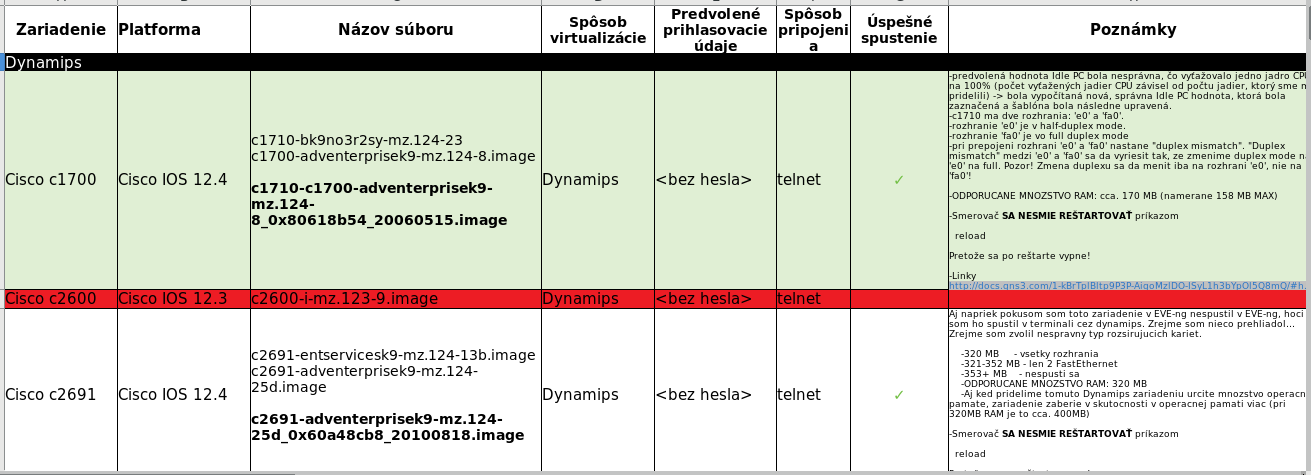
\includegraphics[width=1\textwidth,trim={0.1cm 0.3cm 0.1cm 0.2cm},clip]{sumarny_prehlad_testovanie_spustitelnosti}
    \caption{Tabuľkový dokument s výsledkami testovania spustiteľnosti}
    \label{obr:sumarny_prehlad_testovanie_spustitelnosti}
\end{figure}
}

\begin{longtabu} to \textwidth {| X[2.5,l,m] | X[5.0,l,m] |}
\caption{Popis stĺpcov v sumárnom prehľade zariadení}
\label{tab:sumarny_prehlad_stlpce} \\
\hline
    \multicolumn{1}{|c|}{\textbf{Stĺpec}} & \multicolumn{1}{|c|}{\textbf{Popis}} \\
\hline
    \textbf{Zariadenie} & \makecell[lc]{Názov alebo modelové označenie zariadenia.} \\
\hline
    \textbf{Platforma} & \makecell[lc]{Názov a verzia operačného systému zariadenia.} \\
\hline
    \textbf{Názov súboru} & \makecell[lc]{Pomenovanie zariadenia na serveri.} \\
\hline
    \textbf{Spôsob virtualizácie} & Hypervízor, pod ktorým zariadenie môže byť spustené. \\
\hline
    \textbf{\makecell[lc]{Predvolené prihlasovacie \\ údaje}} & Predvolené prihlasovacie meno a heslo, ak to zariadenie vyžaduje. \\
\hline
    \textbf{Spôsob pripojenia} & \makecell[lc]{Protokol, ktorý sa používa na vzdialenú konfiguráciu \\ zariadenia.} \\
\hline
    \textbf{Úspešné spustenie} & Informácia, či sa zariadenie v topológii spustilo. \\
\hline
    \textbf{Poznámky} & \makecell[lc]{Bližší popis správania sa daného zariadenia, popr. \\ problémy pri používaní zariadenia a ich možné riešenie. \\ Ďalej sa v ňom môžu nachádzať niektoré podporované \\ technológie a internetové odkazy ako zdroj pre informácie \\ uvádzané pre dané zariadenie. V časti v časti\\ \emph{Pridanie zariadenia} sú uvedené odkazy na pridanie\\ zariadenia do nástroja EVE-ng.} \\
\hline
\end{longtabu}

Ďalšie stĺpce slúžia pre prieskum spustiteľnosti zariadení v rôznych nástrojoch nasadených na rôznych platformách.

Pokiaľ sme zistili, že protokol vzdialeného prístupu sa odlišuje od predvoleného protokolu v šablóne na EVE-ng serveri, túto šablónu sme museli upraviť ručne. Avšak s postupným nárastom testovaných zariadení rástol aj počet úprav v šablónach pre jednotlivé zariadenia. Preto sme sa rozhodli vytvoriť skript (kap. \ref{chap:cd} bod \ref{item:uprava_sablon_skript}), ktorý by celý proces automatizoval. Tento skript na úpravu šablón upravuje jednotlivé atribúty konkrétnym zariadeniam. Výsledky testovania sa prejavili v skripte na úpravu šablón, v ktorom boli nastavené atribúty pre protokol na vzdialený prístup k zariadeniam, príp. vlastnosti rozširujúcich kariet zariadení.





\subsection{Testovanie systémových požiadaviek}
\label{chap:testovanie_zariadeni_benchmark}

Testovanie systémových požiadaviek zariadení bolo realizované na fyzickom EVE-ng serveri. Tento druh testovania bol dôležitý preto, aby sme mohli danému zariadeniu nastaviť dostatočné technické parametre, ktoré boli zmerané nástrojmi na meranie systémových prostriedkov. Tak zaistíme jeho plynulý chod a predídeme rôznym komplikáciám počas používania vo vyučovaní. Tieto parametre sú uložené v šablóne pre dané zariadenie.

Úprava šablón je realizovaná skriptom, po ktorého vykonaní sa príslušným zariadeniam zmenia konkrétne technické parametre v šablóne. Po úprave šablón sa zmeny prejavia okamžite a po pridaní zariadenia do topológie, kedy sa jeho parametre automaticky nastavia na správne hodnoty. Pre vybrané zariadenia boli merané tieto veličiny:

\begin{itemize}[noitemsep]
    \item Vyťaženie procesora
    \item Využitie operačnej pamäte
    \item Vyťaženie pevného disku
\end{itemize}

Vyťaženie procesora bolo merané z dôvodu jeho intenzívnej činnosti hlavne počas spúšťania zariadení, ale môže byť vyťažovaný aj po dokončení spúšťania. Na základe toho budeme vedieť určiť, koľko zariadení budeme môcť v topológii spustiť naraz, a koľko už spustených zariadení zvládne server spravovať celkovo. Pri meraní vyťaženia procesora bolo merané celkové vyťaženie aj vyťaženie jednotlivých jadier procesora.

Operačná pamäť je najviac využitá po dokončení spúšťania zariadenia. Kapacita operačnej pamäte ovplyvňuje celkový počet spustených zariadení na serveri. Meranie jej vyťaženia je pomerne jednoduché pre celý systém, ale pre tieto účely bolo potrebné s vysokou presnosťou vedieť, koľko operačnej pamäte využíva iba konkrétne zariadenie.

Na meranie využitia operačnej pamäte boli použité dva nástroje: \texttt{ps} a \texttt{ps\_mem}. Prvý z nich už bol na EVE-ng serveri prítomný, druhý bolo potrebné nainštalovať dodatočne. Na meranie boli použité dva nástroje, aby sa navzájom výsledky oboch nástrojov medzi sebou validovali.

Disk je najviac vyťažený predovšetkým pri spúšťaní zariadenia, ale môže byť vyťažený aj po dokončení spúšťania. Vyťaženie disku bolo do merania zahrnuté, aby sme vedeli odhadnúť, do akej miery je spúšťanie a beh zariadení ovplyvnené načítavaním zariadenia z pevného disku.

Z merania bola vynechaná frekvencia procesora a vyťaženie sieťového rozhrania. Frekvencia procesora bola vynechaná, lebo procesor podľa príkazu \texttt{watch lscpu | grep "MHz"} striedal iba dve frekvencie, 2000.000 MHz (minimálna frekvencia) a 2333.000 MHz (maximálna frekvencia), nezávisle na celkovom vyťažení procesora.

Vyťaženie sieťovej karty je zanedbateľné pri meraní výkonnosti jednotlivých zariadení, keďže sa sieť využíva iba na interakciu používateľa s klientskou aplikáciou, čo vytvára zanedbateľnú záťaž.

Na monitorovanie vybraných veličín sú určené rôzne nástroje a stratégie. Mohli sme napr. vytvoriť skript, ktorý by pomocou viacerých špecializovaných nástrojov meral vyťaženie jednotlivých prvkov systému, alebo použiť nástroj, ktorý je schopný monitorovať široké spektrum systémových zdrojov. Zvažovali sme tieto nástroje:

\begin{description}[noitemsep]
    \item [iotop] monitorovanie procesov podľa využitia disku
    \item [nmap] monitorovanie sieťovej prevádzky
    \item [nethogs] monitorovanie procesov podľa využitia sieťového rozhrania
    \item [dstat] monitorovanie rôznych systémových prostriedkov v CLI
    \item [sysstat] rovnako, ako nástroj \emph{dstat}
    \item [netdata] monitorovanie rôznych systémových prostriedkov cez webové rozhranie
\end{description}

Z uvedených nástrojov sme sa rozhodli použiť nástroj \emph{dstat}. Hlavným dôvodom, prečo sme sa rozhodli ďalej používať a upravovať tento nástroj a uprednostniť ho pred ostatnými nástrojmi, bolo predovšetkým ukladanie ziskaných údajov do CSV súboru. Dáta sa do CSV súboru zapisovali každú sekundu. Následne sme si vytvorili tabuľkový dokument, ktorý vyhodnocoval namerané dáta z CSV súboru. Vyhodnocovaním nameraných údajov sa budeme bližšie zaoberať v časti \ref{chap:testovanie_zariadeni_benchmark_vyhodnotenie}.

Nástroj \emph{dstat} však bolo potrebné upraviť tak, aby zisťoval využitie operačnej pamäte iba pre zariadenia v EVE-ng topológii, nie celého systému.

Pre tento účel sme vytvorili kópiu nástroja \emph{dstat} s názvom \emph{dstat\_custom}. V tejto kópii sme následne upravovali jeho zdrojový kód pre naše potreby. Nástroj \emph{dstat} bol vytvorený v programovacom jazyku Python.

Nástroj \emph{dstat\_custom} bol upravený tak, že meria využitie operačnej pamäte pre zariadenie v EVE-ng topológii nástrojmi \emph{ps} a \emph{ps\_mem}. Obidva príkazy merajú tú istú množinu procesov patriacu spustenému zariadeniu resp. spusteným zariadeniam topológii, aby sme mohli hodnoty oboch nástrojov medzi sebou porovnať. Hodnoty namerané obomi nástrojmi by mali byť približne rovnaké na to, aby sme mohli výsledky považovať za validné.

Vo výslednom CSV súbore vytvorenom nástrojom \emph{dstat\_custom} sa stĺpce \emph{used} a \emph{buffered} v časti \emph{memory usage} nahradia stĺpcami \emph{MemUsed-ps} a \emph{MemUsed-ps\_mem}.

Aby nástroj \emph{dstat\_custom} fungoval správne, musia byť nainštalované balíčky \emph{dstat}, \emph{ps\_mem} a \emph{sultan}. Význam prvých dvoch balíčkov už bol v tejto časti vysvetlený. Balíček \emph{sultan} slúžil na vykonávanie terminálových príkazov zvnútra Python programu.

Výsledky z merania systémových požiadaviek je takisto možné použiť v iných nástrojoch na sieťovú virtualizáciu. Pokiaľ existuje ekvivalentný typ zariadenia aj v inom nástroji, je odporúčané aplikovať namerané systémové parametre do jeho šablóny za predpokladu, že je pre zariadenie použitý rovnaký spôsob virtualizácie resp. hypervízor, napr. QEMU/KVM, Docker a pod.





\subsubsection{Metodika}

Najprv bol vytvorený zoznam vybraných zariadení, ktorých systémové požiadavky sme sa rozhodli testovať. Ten sa nachádza v kapitole \ref{chap:cd} v bode \ref{item:benchmarking_list} a na obr. \ref{obr:zoznam_zariadeni_test_sys_poziadaviek}. Zoznam zariadení bol vytvorený na základe kapitoly \ref{chap:analyza_vyucovania} - \nameref{chap:analyza_vyucovania}, keďže malo zmysel testovať iba tie zariadenia, ktoré by mohla katedra použiť vo vyučovaní.

\afterpage{
\begin{figure}
    \centering
    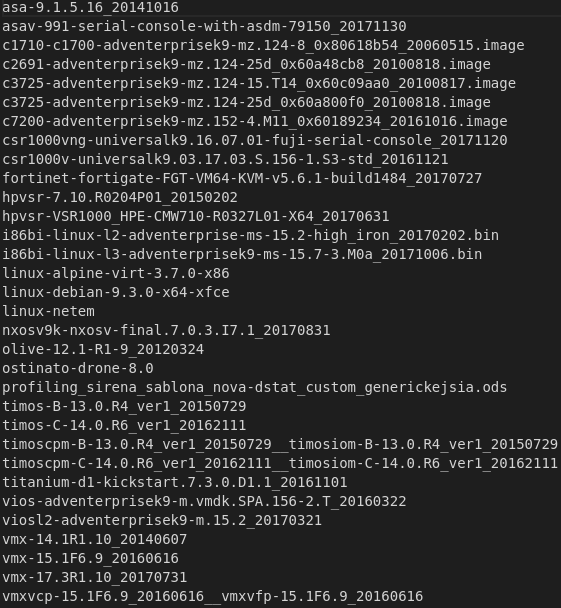
\includegraphics[width=0.7\textwidth,trim={0cm 8.1cm 0cm 0cm},clip]{zoznam_zariadeni_test_sys_poziadaviek}
    \caption{Textový dokument so zoznamom zariadení pre testovanie ich systémových požiadaviek}
    \label{obr:zoznam_zariadeni_test_sys_poziadaviek}
\end{figure}
}

Meranie systémových zdrojov zariadenia bolo vykonané nástrojom \emph{dstat\_custom}. Pred začiatkom každého merania bolo potrebné vykonať kroky, ktoré zvyšujú konzistenciu a presnosť výsledkov a reprezentujú najhoršie možné podmienky pre beh zariadenia. Všetky zariadenia sú uložené na rovnakom pevnom disku ako operačný systém.

Pred začatím merania výkonnosti každého zariadenia bolo v rámci úvodných krokov vypnuté používanie \emph{swap} partície a vyprazdnené vyrovnávacie časti operačnej pamäte (\emph{cache} a \emph{buffer}).

Na EVE-ng serveri bola počas celého merania vypnutá funkcia UKMS (Universal Kernel Samepage Merging). UKSM je mechanizmus, ktorý umožňuje šetriť využitie operačnej pamäte, keď je spustených viacero zariadení rovnakého typu. Ak je ale UKMS aktívne a spustíme viac ako 10 QEMU zariadení, ich výkon by mohol byť v dôsledku tohto mechanizmu znížený \cite{eve_ng_faq}.

\noindent
Meranie systémových požiadaviek zariadenia prebiehalo nasledovne:

\begin{enumerate}[noitemsep]
    \item Do EVE-ng predpripravenej prázdnej topológie pridáme zariadenie, ktoré chceme testovať.
    \item \label{nastavenie_sys_param} Nastavíme mu maximálne množstvo operačnej pamäte, s ktorým je zariadenie schopné úspešne sa spustiť. Ak je to možné, nastavíme počet procesorov na 1 CPU - tak bude záťaž na procesor minimalizovaná.
    \item Vykonáme vyššie uvedené úvodné kroky pred meraním.
    \item Nástrojom \emph{dstat\_custom} spustíme sledovanie systémových prostriedkov, ktorý bude ukladať namerané údaje do súboru.
    \item Spustíme zariadenie.
    \item Z nástroja zistíme čas spustenia zariadenia a zapíšeme si ho do osobitného súboru napr. \emph{boot\_time.txt}.
    \item Pripojíme sa na konzolu zariadenia. Počkáme, kým neuvidíme interaktívny príkazový riadok (CLI) alebo výzvu na prihlásenie.
    \item Ak je to nutné, po úspešnom spustení zariadenia sa naň prihlásime.
    \item Akonáhle uvidíme interaktívny príkazový riadok (CLI), do súboru \emph{boot\_time.txt} si uložíme čas, v ktorom zariadenie dokončilo svoje spúšťanie. 
    \item Zariadenie necháme 1-3 minúty stabilizovať.
    \item Ukončíme sledovanie systémových prostriedkov.
    \item Zastavíme zariadenie a odstránime ho z topológie.
\end{enumerate}

Pokiaľ sa vyskytli komplikácie so spúšťaním alebo behom zariadenia, vrátili sme sa na krok \ref{nastavenie_sys_param} a stanovili sme pre zariadenie iné systémové parametre. Systémové parametre zariadenia sme menili dovtedy, kým sa zariadenie nespustilo a odozva z klávesnice z jeho konzoly bola prijateľná. Podrobnejší popis rôznych konfigurácii systémových parametrov pre konkrétne zariadenia je k dispozícii v kapitole \ref{chap:cd} v bode \ref{item:sumarny_prehlad_zariadeni}

Po skončení merania vznikli dva nové súbory: súbor s nameranými údajmi a súbor s trvaním spúšťania zariadenia. Tieto súbory tvorili vstup pre tabuľkový súbor na vyhodnocovanie nameraných údajov pre zariadenie, ktorému sa venujeme v nasledujúcej časti.

Po ukončení merania všetkých zariadení môžeme znova zapnúť "swap" partíciu.





\subsubsection{Vyhodnotenie}
\label{chap:testovanie_zariadeni_benchmark_vyhodnotenie}

Po vytvorení súboru s nameranými údajmi a súboru s trvaním spúšťania zariadenia môžeme vložiť ich údaje do tabuľkového dokumentu. Na základe vstupných údajov sa automaticky prepočítajú výstupné hodnoty vo všetkých tabuľkách tohto dokumentu. Nižšie je opísaný priebeh vyhodnotenia nameraných údajov:

\begin{enumerate}[noitemsep]
    \item Do hárku \emph{SuroveUdaje} vložíme dáta namerané nástrojom \emph{dstat\_custom}.
    \item Do hárku \emph{VstupVystup} vložíme tieto údaje
    \begin{enumerate}[noitemsep]
        \item Do poľa \emph{Start} zadáme čas, kedy sme zariadenie spustili.
        \item Do poľa \emph{Stop} zadáme čas, kedy zariadenie dokončilo svoje spúšťanie a zobrazilo interaktívny príkazový riadok (CLI).
        \item Do poľa \emph{Množstvo voľnej RAM na serveri (MB)} zadáme množstvo voľnej operačnej pamäte na EVE-ng serveri v stave pokoja.
    \end{enumerate}
\end{enumerate}

Po zadaní spomenutých vstupných údajov tabuľkový dokument poskytne v hárku \emph{VstupVystup} odpovede na tieto otázky:

\begin{itemize}[noitemsep]
    \item Čas spúšťania - čas potrebný na dokončenie spúšťania zariadenia
    \item Odhadované množstvo operačnej pamäte pre jedno zariadenie / topológiu (MB)
    \item Odhadovaný počet zariadení, ktoré je možné naraz spustiť na základe celkového vyťaženia CPU
    \item Odhadovaný počet sputených zariadení na základe celkového vyťaženia CPU
    \item Odhadovaný počet sputených zariadení na základe voľnej RAM
\end{itemize}

Od všetkých vstupných údajov boli pred ďalším spracovaním odčítané namerané hodnoty z pokojového stavu EVE-ng servera.

Výsledky merania systémových požiadaviek zariadení reprezentujú najhorší možný scenár behu zariadenia.

Výsledky testovania vybraných zariadení sú prítomné v kapitole \ref{chap:cd} v časti \ref{item:all_benchmarks} \emph{eve-ng/profiling\_and\_benchmarking\_results}. Na obr. \ref{obr:testovanie_systemovych_poziadaviek_sablona} je ako príklad znázornený výstup tabuľkového súboru pre systémové požiadavky virtuálneho smerovača \emph{Cisco 7200}.

\begin{figure}
    \centering
    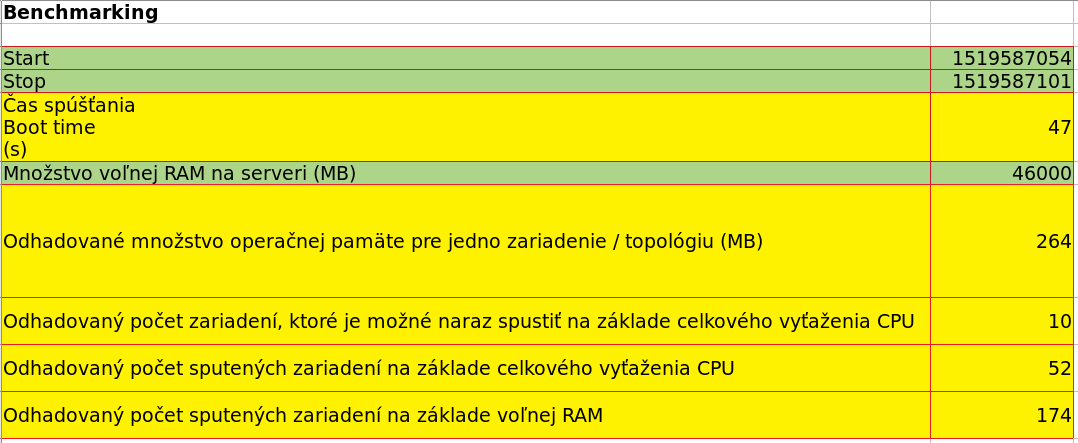
\includegraphics[width=1\textwidth,trim={0cm 0.1cm 0.1cm 0cm},clip]{testovanie_systemovych_poziadaviek_sablona}
    \caption{Tabuľkový dokument s nameranými systémovými požiadavkami}
    \label{obr:testovanie_systemovych_poziadaviek_sablona}
\end{figure}


Podľa tabuľkového dokumentu bolo pre každé zariadenie nastavené množstvo operačnej pamäte a počet CPU v skripte na úpravu šablón. Zariadenie vďaka tomu môžeme pridávať do topológie bez toho, aby sme museli premýšľať, či má nastavené dostatočné systémové parametre.

Celý proces merania systémových požiadaviek zariadení je bližšie vysvetlený v kapitole \ref{chap:cd} v bode \ref{item:benchmarking_popis}





\subsection{Testovanie technológii}
\label{chap:testovanie_technologii}

V tejto časti využijeme poznatky z kapitoly \ref{chap:analyza_vyucovania} - \nameref{chap:analyza_vyucovania} a použijeme ich na testovanie, či vybrané zariadenia podporujú témy vyučované na katedre. Testované boli iba podporované technológie Cisco zariadení, keďže tie sa používajú vo vyučovaní najviac.

Cieľom testovania technológii je zistiť, do akej je možné použiť virtuálne zariadenia pri vyučovaní takých tém, na ktoré boli doposiaľ použité fyzické zariadenia alebo virtualizačné riešenia s užším rozsahom podporovaných technológii. Jednalo sa najmä o podporu prepínacích technológii na predmetoch \emph{Pokročilé prepínanie v informačno-komunikačných sieťach} (CCNP Switching) a \emph{Počítačové siete 1} (CCNA 2 + prepínacie technológie). Prioritné boli testované témy vyučované na CCNP kurze, keďže prepínacie technológie v CCNP kurze zahŕňajú aj tie zo CCNA.





\subsubsection{Metodika}

Na testovanie podporovaných technológii vybraných zariadení bol vytvorený skript, ktorý je dostupný v kapitole \ref{chap:cd} v bode \ref{item:cisco_feature_testing_skript} a znázornený na obr. \ref{obr:skript_testovanie_podporovanych_technologii_cisco}. Skript sa skladal z viacerých skupín konfiguračných príkazov, pričom každá skupina mala za úlohu testovať podporu konkrétnej technológie na zariadení. Časti tohto skriptu boli postupne zadávané do konfigurácie zariadenia.

Nižšie je uvedený zoznam testovaných zariadení pre tento účel:

\begin{itemize}[noitemsep]
    \item Cisco IOL prepínač
    \item Cisco vIOS prepínač
    \item Cisco 3725 s EtherSwitch modulom
    \item Cisco 7200
    \item Cisco IOL smerovač
    \item Cisco vIOS smerovač
    \item Cisco CSR
    \item Cisco CSR-ng
\end{itemize}

\begin{figure}
    \centering
    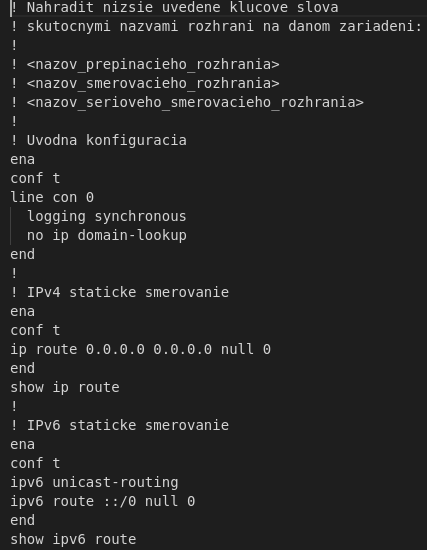
\includegraphics[width=0.35\textwidth,trim={0cm 0cm 5cm 4.65cm},clip]{skript_testovanie_podporovanych_technologii_cisco}
    \caption{Skript na testovanie podporovaných technológií pre Cisco zariadenia}
    \label{obr:skript_testovanie_podporovanych_technologii_cisco}
\end{figure}


\subsubsection{Vyhodnotenie}
\label{chap:testovanie_technologii_vyhodnotenie}

Po vykonaní konfiguračných príkazov zo skriptu bolo potrebné vyhodnotiť, či a do akej miery je testovaná technológia na danom zariadení podporovaná. Technológia bola označená ako podporovaná vtedy, ak príkaz nevypísal žiadne chybové hlásenie. V opačnom prípade sa testovali alternatívne konfigurácie. Ak sa ani žiadna z alternatívnych konfigurácii nevykonala úspešne, technológia bola vyhodnotená ako nepodporovaná. Výsledky testovania technológii sú dostupné v kapitole \ref{chap:cd} v bode \ref{item:zoznam_technologii_s_podporou_zariadeni} a ukážka tohto tabuľkového dokumentu je znázornená na obr. \ref{obr:zoznam_technologii_s_podporou_zariadeni}. V stĺpci \emph{Technológia} sa nachádza názov vyučovanej témy. Stĺpec \emph{Predmety} obsahuje skratku predmetu, na ktorej je táto téma vyučovaná. Podporované vyučované témy jednotlivých testovaných zariadení sú farebne odlíšené, popr. doplnené krátkym komentárom.

%\afterpage{
\begin{figure}
    \centering
    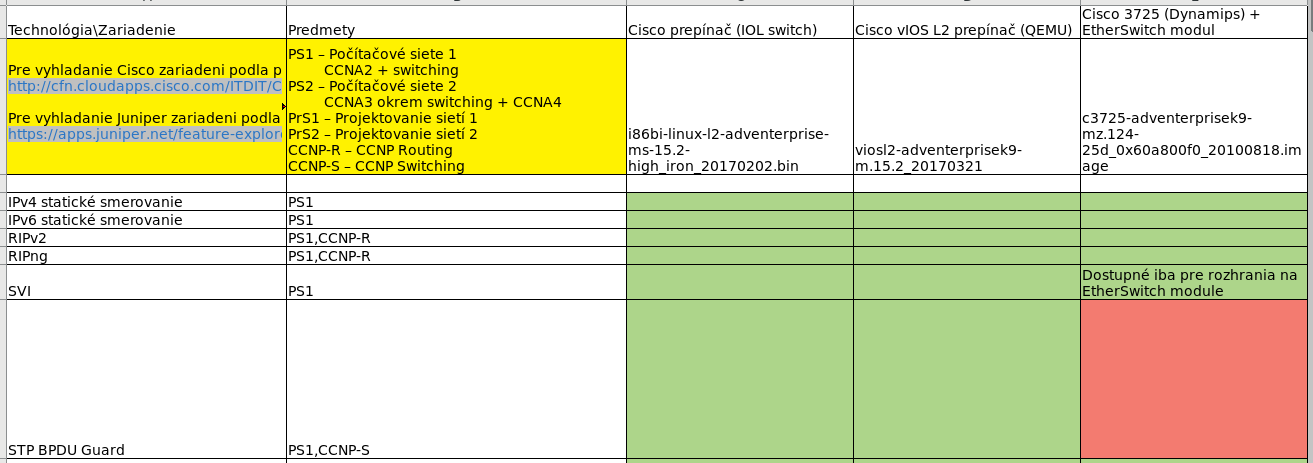
\includegraphics[width=1\textwidth,trim={0.2cm 0.15cm 0.15cm 0.15cm},clip]{zoznam_technologii_s_podporou_zariadeni}
    \caption{Tabuľkový súbor s podporovanými technológiami pre jednotlivé zariadenia}
    \label{obr:zoznam_technologii_s_podporou_zariadeni}
\end{figure}
%}

Zo spomenutého súboru vyplýva, že prepínacie technológie sú dostupné iba na zariadeniach \emph{Cisco IOL prepínač} a \emph{Cisco vIOS prepínač}. EtherSwitch modul na prepínači Cisco 3725 síce podporoval niektoré prepínacie technológie, ale bolo ich výrazne menej. Prepínacími technológiami sa zaoberajú hlavne predmety Počítačové siete 1 a Pokročilé prepínanie v informačno-komunikačných sieťach.

Špeciálne postavenie má \emph{Cisco IOL smerovač}, ktorý ako jediný v EVE-ng obsahuje sériové rozhrania, preto aj ako jediný v EVE-ng podporuje Point-to-point technológie. Tento druh smerovača je dôležité pre predmety Počítačové siete 1/2 a Pokročilé prepínanie/smerovanie v informačno-komunikačných sieťach. Ďalšou zvláštnosťou je, že v EVE-ng nie je možné odchytávať prevádzku pre sériové rozhranie. Zaujímavosťou je, že zo všetkých testovaných smerovačov mal najnižšie spotrebu operačnej pamäte, cca 250 MB. V nástroji EVE-ng je prítomný Cisco IOL smerovač z roku 2017 s operačným systémom \emph{IOS 15.7-3.M0a}.

Ukázalo sa, že smerovače \emph{Cisco 3725}, \emph{Cisco 7200}, \emph{Cisco IOL smerovač} a \emph{Cisco vIOS smerovač} majú veľmi podobnú množinu funkcií, až na malé odchýlky. Cisco 3725 s EtherSwitch modulom ako jediný spomedzi nich podporuje SVI, PortFast, 802.1Q Trunk, VTPv1/v2, STP, HSRP a HSRPv2 (obe pre IPV4), VRRPv2, SPAN a IGMP Snooping. avšak nepodporuje GLBP IPv6 ani EIGRP IPv6. Prepínacie technológie sú dostupné iba pre rozhrania v EtherSwitch module. Spomínané 4 smerovače je možné použiť v topológiách pre uzly, ktoré nevyžadujú sériové prepojenia v rámci ľubovoľného predmetu.

Smerovače \emph{Cisco CSR} a \emph{Cisco CSR-ng} sú vhodné na pokročilejšie sieťové technológie, ako napr. VPLS, vyučovaných na predmetoch Projektovanie sietí 1/2. Zvláštnosťou je chýbajúca podpora GLBP pre IPv6 na \emph{Cisco CSR}. Zaujímavou je podpora niektorých prepínacích technológii pre Cisco CSR-ng a v menšej miere pre Cisco CSR, hoci je ich ešte menej, ako pri smerovači Cisco 3725. Nevýhodou oboch smerovačov, v porovnaní s ostatnými šiestimi, sú ich vyššia spotreba operačnej pamäte, cca 4,5 GB.

Výsledky tohto prieskumu boli použité v poslednej fáze projektu - \nameref{chap:nasadenie_do_vyucovania}, ktorej sa venujeme v kapitole \ref{chap:nasadenie_do_vyucovania}. Vyhodnotenie slúži iba na odhad, ktoré zariadenia majú najväčšiu pravdepodobnosť využitia na danom predmete. V prípade, že má predmet v zozname viacero zariadení, treba sa na základe ďalších kritérií rozhodnúť, ktoré z nich budú použité v topológii. Môžeme napr. brať do úvahy iné vyučované témy v topológii, systémové požiadavky zariadenia, iné technické obmedzenia zariadenia a pod. V každom prípade je potrebné pred vytvorením akejkoľvek topológie použiť zoznam podporovaných funkcií pre zariadenia v kapitole \ref{chap:cd} v bode \ref{item:zoznam_technologii_s_podporou_zariadeni} 